\documentclass[11pt]{article}
%\usepackage[14pt]{extsizes} % для того чтобы задать нестандартный 14-ый размер шрифта
%\usepackage[utf8]{inputenc}
\usepackage{mathtext}
\usepackage[english, russian]{babel}
\usepackage{amsmath}
\usepackage{amsfonts}
\usepackage{float}
\usepackage[margin=0.8in]{geometry}
\usepackage{multirow}
\usepackage{graphicx}
\usepackage[utf8x]{inputenc} % указать кодировку русского текста
\usepackage{fancyhdr}
\usepackage{indentfirst} % отступ в первой строке абзаца
\usepackage{wrapfig}
\usepackage{placeins}
\usepackage{wrapfig}
\usepackage{caption}
\usepackage{amssymb}
\usepackage{mathtools}
\usepackage[thinc]{esdiff}
\usepackage{cmap}
\usepackage[table,xcdraw]{xcolor}

\usepackage{breqn}

\pagestyle{fancy}
\begin{document}
\begin{titlepage}
\begin{center}
%\vspace*{1cm}
\large{\small ФЕДЕРАЛЬНОЕ ГОСУДАРСТВЕННОЕ АВТОНОМНОЕ ОБРАЗОВАТЕЛЬНОЕ\\ УЧРЕЖДЕНИЕ ВЫСШЕГО ОБРАЗОВАНИЯ\\ МОСКОВСКИЙ ФИЗИКО-ТЕХНИЧЕСКИЙ ИНСТИТУТ\\ (НАЦИОНАЛЬНЫЙ ИССЛЕДОВАТЕЛЬСКИЙ УНИВЕРСИТЕТ)\\ ФИЗТЕХ-ШКОЛА РАДИОТЕХНИКИ И КОМПЬЮТЕРНЫХ ТЕХНОЛОГИЙ}
\vfill
\line(1,0){430}\\[1mm]
\huge{Лабораторная работа 3.6.1}\\
\huge\textbf{Спектральный анализ электрических сигналов.}\\
\line(1,0){430}\\[1mm]
\vfill
\begin{flushright}
\normalsize{Устюжанина Мария}\\
\normalsize{\textbf{Группа Б01-107}}\\
\end{flushright}
\end{center}
\end{titlepage}
\fancyhead[L] {Работа 3.6.1}

\par \textbf{Цель работы:} Изучить спектральный состав периодических электричeских сигналов.

\par \textbf{В работе используются:} Анализатор спектра, генератор прямоугольных импульсов и сигналов специальной формы,осциллограф.

\section{Теоретическая часть:}

\subsection*{Разложение сложных сигналов на периодические колебания}
Метод для описания сигналов. Для него используется разложение в сумму синусов и косинусов с различными аргументами или, как чаще его называют, \textit{разложение в ряд Фурье}.

Пусть задана функция $f(t)$, которая периодически повторяется с частотой $\Omega_1 = \dfrac{2\pi}{T}$, где $T$ --- период повторения импульсов. Её разложение в ряд Фурье имеет вид 
\begin{equation}
f(t) = \dfrac{a_0}{2} + \sum\limits_{n = 1}^{\infty}\left[a_n \cos \left(n \Omega_1t\right) + b_n \sin \left(n \Omega_1t\right)\right]
\end{equation}
или
\begin{equation}
f(t) = \dfrac{a_0}{2} + \sum\limits_{n = 1}^{\infty}A_n \cos \left(n\Omega_1t-\psi_n\right)
\end{equation}
Если сигнал четен относительно $t=0$, так что $f(t) = f(-t)$ в тригонометрической записи остаются только косинусные члены. Для нечетной наоборот.

Коэффициенты определяются по формуле
\begin{equation}
\begin{array}{c}
a_n  = \dfrac{2}{T}\int\limits_{t_1}^{t_1+T}f(t)\cos\left(n \Omega_1 t\right) dt\\
\\
b_n = \dfrac{2}{T}\int\limits_{t_1}^{t_1+T}f(t)\sin\left(n \Omega_1 t\right) dt
\end{array}
\end{equation}
Здесь $t_1$ --- время, с которого мы начинаем отсчет.

Сравнив формулы $(1)$ и $(2)$ можно получить выражения для $A_n$  и $\psi_n$:
\begin{equation}
A_n = \sqrt{a_n^2+b_n^2};\psi_n = \arctan \dfrac{b_n}{a_n}
\end{equation}
\subsection*{Периодическая последовательность прямоугольных импульсов}
Введем некоторые величины:
\[\Omega_1 = \dfrac{2\pi}{T}, \]
где $T$ --- период повторения импульсов.

Коэффициенты при косинусных составляющих будут равны
\begin{equation}
a_n = \dfrac{2}{T}\int\limits_{-\tau/2}^{\tau/2}V_0\cos\left(n\Omega_1 t\right)dt = 2V_0\dfrac{\tau}{T}\dfrac{\sin\left(n\Omega_1\tau/2\right)}{n\Omega_1\tau/2} \sim \dfrac{\sin x}{x}
\end{equation}

Здесь $V_0$ - амплитуда сигнала.

Поскольку наша функция четная, то $b_n = 0$. 

Пусть у нас $\tau$ кратно $T$. Тогда введем ширину спектра, равную $\Delta \omega$ --- расстояние от главного максимума до первого нуля огибающей, возникающего, как нетрудно убедится при $n = \dfrac{2\pi}{\tau \Omega_1}$. При 
этом
\begin{equation}
\Delta \omega \tau \simeq 2\pi \Rightarrow \Delta \nu \Delta t \simeq 1
\end{equation}
\subsection*{Периодическая последовательность цугов}
Функция $f(t)$ снова является четной относительно $t = 0$. Коэффициент при $n$-ой гармонике согласно формуле $(3)$ равен
\begin{equation}
a_n = \dfrac{2}{T}\int\limits_{-\tau/2}^{\tau/2}V_0 \cos \left(\omega_0t\right) \cdot \cos\left(n \Omega_1t\right)dt = V_0 \dfrac{\tau}{T}\left( \dfrac{\sin\left[\left(\omega_0 - n \Omega_1\right)\dfrac{\tau}{2}\right]}{\left( \omega_0 - n \Omega_1\right) \dfrac{\tau}{2}} + \dfrac{\sin\left[\left(\omega_0 + n \Omega_1\right)\dfrac{\tau}{2}\right]}{\left( \omega_0 + n \Omega_1\right) \dfrac{\tau}{2}}\right)
\end{equation}
\subsection*{Амплитудно-модулированные колебания}
Рассмотрим гармонические колебания высокой частоты $\omega_0$, амплитуда которых медленно меняется по гармоническому закону с частотой $\Omega \ll \omega_0$.
\begin{equation}
f(t) = A_0 \left[1+m\cos \Omega t\right] \cos \omega_0 t
\end{equation}
Коэффициентом $m$ называется \textit{глубина модуляции}. При $m < 1$ амплитуда меняется от минимальной $A_{min} = A_0(1-m)$ до максимальной $A_{max} = A_0(1+m)$. Глубина модуляции может быть представлена в виде
\begin{equation}
m = \dfrac{A_{max}-A_{min}}{A_{max}+A_{min}}
\end{equation}
Простым тригонометрическим преобразованием уравнения $(9)$ можно найти спектр колебаний
\begin{equation}
f(t) = A_0 \cos \omega_0t + \dfrac{A_0m}{2} \cos \left(\omega_0 + \Omega\right)t + \dfrac{A_0m}{2}\cos\left(\omega_0 - \Omega\right)t
\end{equation}



\section{Ход работы:}

\subsection{A. Исследование спектра периодической последовательности прямоугольных импульсов}

Исследуем прямоугольные импульсы с \( \nu_{rep} = 1кГц \) и длительностью импульса \( \tau = 100мкс \). Получим на экране спектр сигнала и будем изменять $\tau$ и $\nu_{rep}$, наблюдая как изменяется спектр.

\begin{figure}[H]
    \centering
    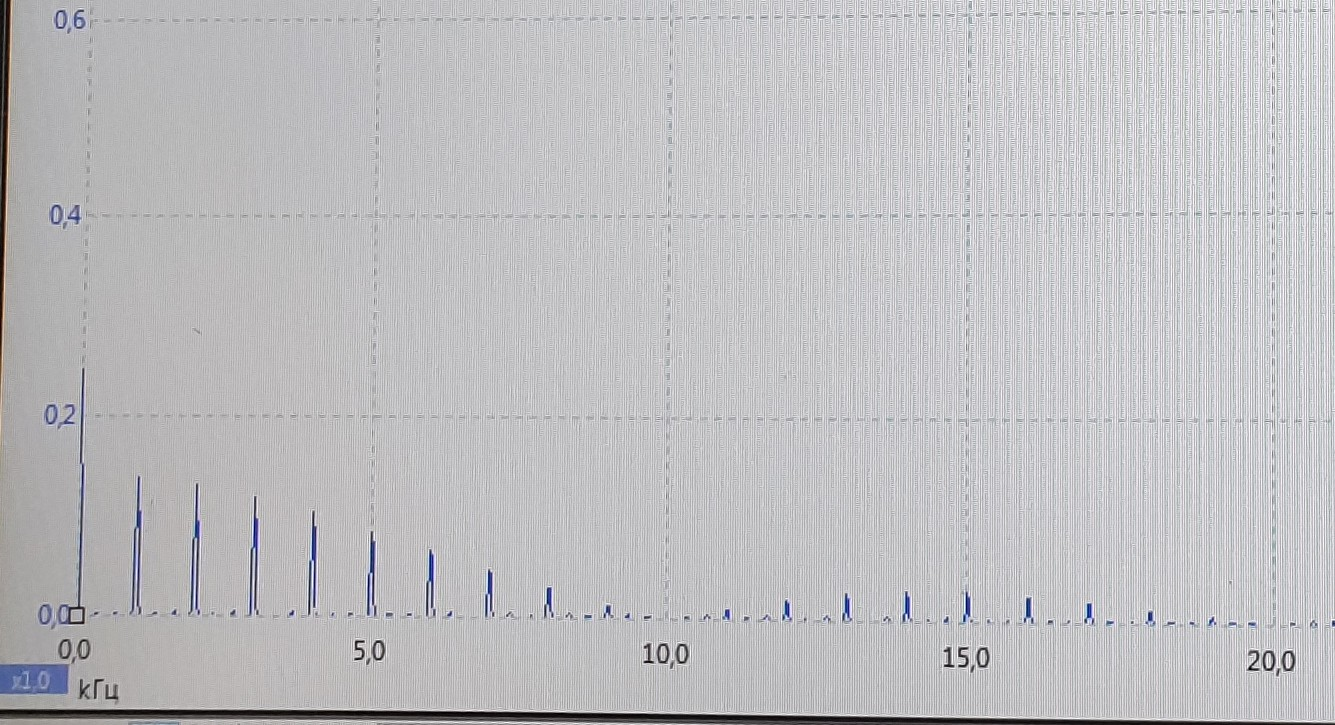
\includegraphics[width=0.8\textwidth]{1.jpg}
    \caption{Спектр при \( \nu_{rep} = 1 кГц, \tau = 100мкс \)}
    \label{spec_1}
\end{figure}

\begin{figure}[H]
    \centering
    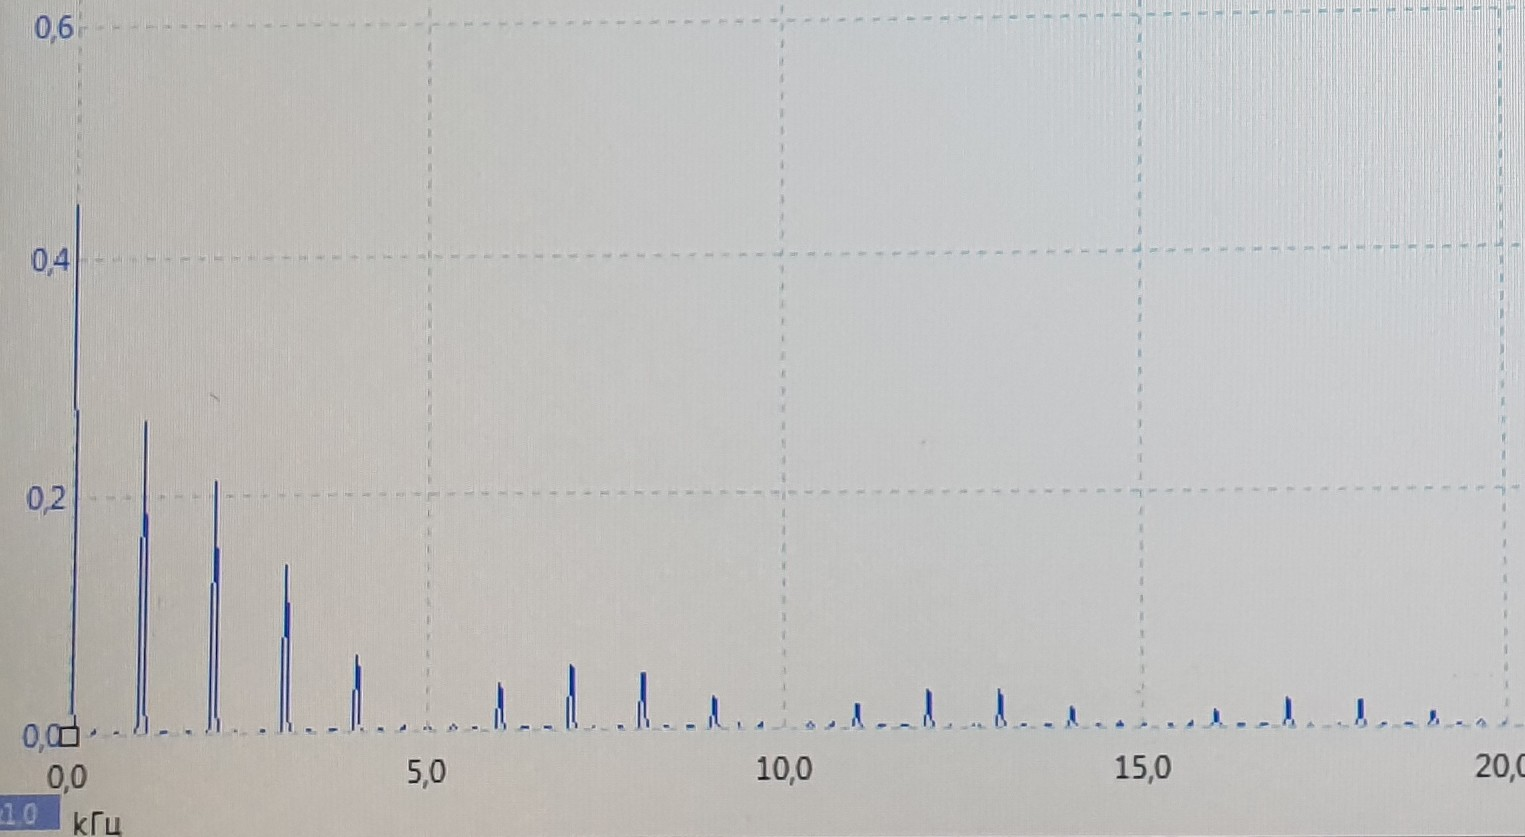
\includegraphics[width=0.8\textwidth]{2.jpg}
    \caption{Спектр при \( \nu_{rep} = 1 кГц, \tau = 200мкс \)} 
    \label{spec_2}
\end{figure}

\begin{figure}[H]
    \centering
    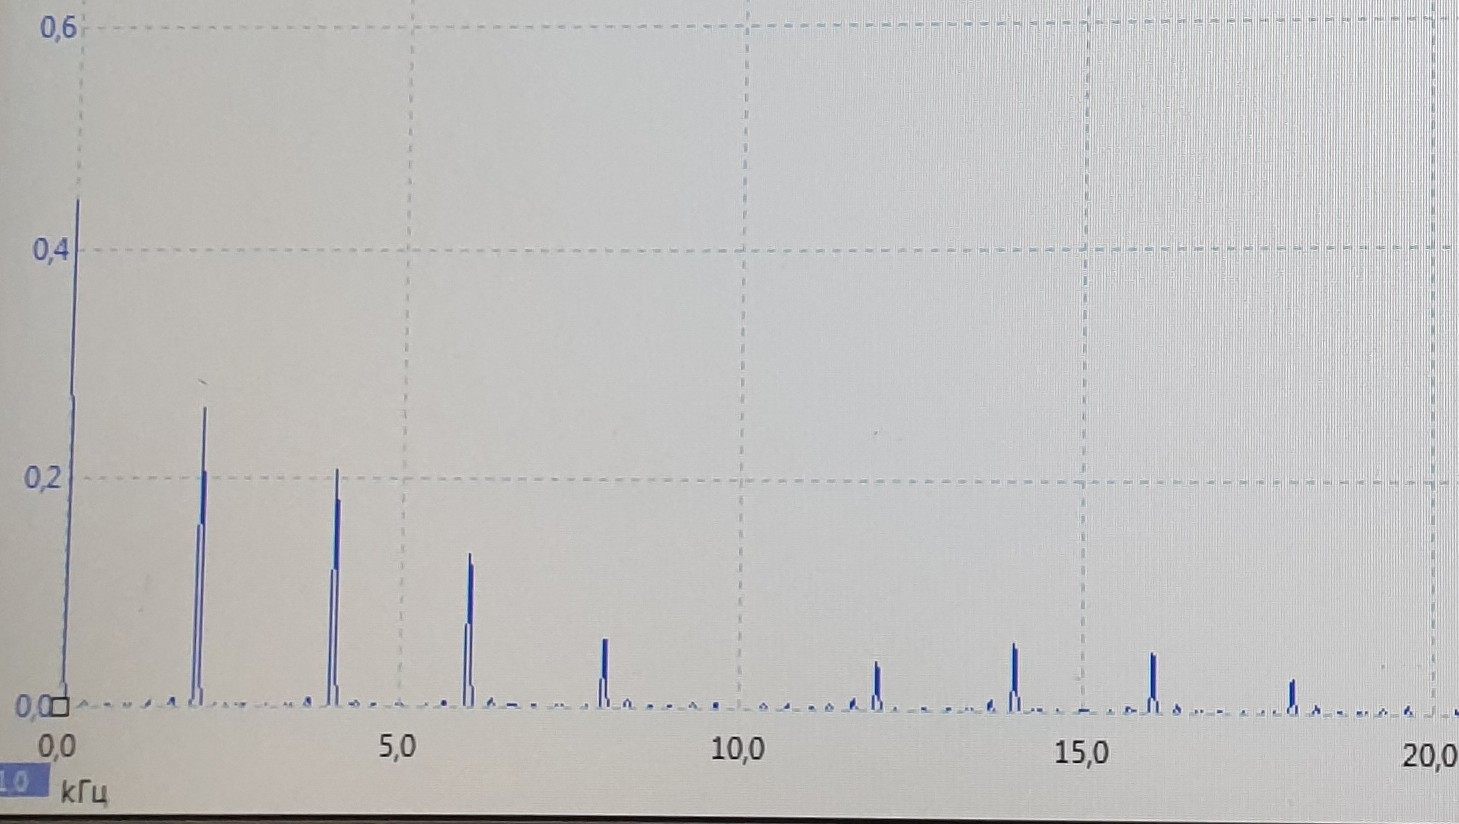
\includegraphics[width=0.8\textwidth]{3.jpg}
    \caption{Спектр при \( \nu_{rep} = 2 кГц, \tau = 100мкс \)} 
    \label{spec_3}
\end{figure}

Исследуем зависимость ширины спектра от длительности импульса при частоте повторения \( \nu_{rep} = 1кГц \)

\begin{table}[H]
    \centering
    \begin{tabular}{|c|c|}
        \hline
        \(\tau\), мкс& \(\Delta\nu\), кГц \\\hline
        40                        & 25                  \\\hline
        60                        & 16                  \\\hline
        80                        & 13                  \\\hline
        100                       & 10                  \\\hline
        120                       & 8                   \\\hline
        140                       & 7                   \\\hline
        160                       & 6                   \\\hline
        180                       & 5.5                \\\hline
        200                       & 5                   \\\hline
    \end{tabular}
\end{table}

Запишем резульаты в таблицу \( \Delta\nu(1/\tau) \):


\begin{table}[H]
    \centering
    \label{tab_dnu_tau}
    \begin{tabular}{|c|c|}
        \hline
        \(1/\tau\), кГц & \(\Delta\nu\), кГц \\\hline
        25    & 25   \\\hline
        16.67 & 16   \\\hline
        12.5  & 13   \\\hline
        10    & 10   \\\hline
        8.33  & 8    \\\hline
        7.14  & 7    \\\hline
        6.25  & 6    \\\hline
        5.56  & 5.50 \\\hline
        5     & 5   \\\hline
    \end{tabular}
\end{table}

Получим график:
\begin{figure}[H]
    \centering
    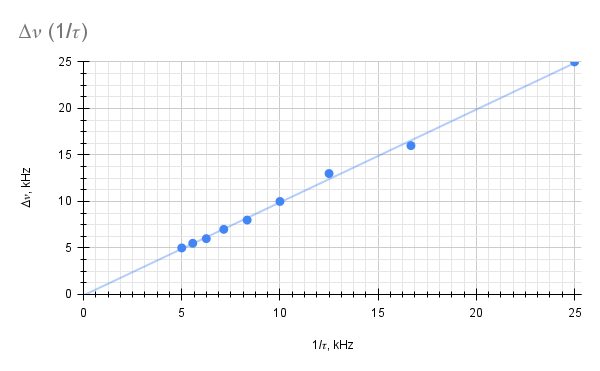
\includegraphics[width=0.8\textwidth]{graf1.png}
    \caption{График \( \Delta\nu(1/\tau) \) для прямоугольных импульсов с \( \nu_{rep} = 1кГц \)}
    \label{pic_dnu_tau}
\end{figure}
Тогда зависимость:

    \[ \Delta\nu = (0.998 \pm 0.016) \cdot \frac{1}{\tau} + (0.094 \pm 0.098) кГц \]

Выполняется соотношение определённости:
\[ \Delta\nu\cdot\tau \simeq 1 \]

\subsection{B. Исследование спктра периодической последовательности цугов гармонических колебаний}

Исследуем последовательность цугов, для этого установим частоту несущей \( \nu_0 = 25кГц \) и получим на экране осциллографа устойчивую картину.

Пронаблюдаем изменение спектра:

\begin{figure}[H]
    \centering
    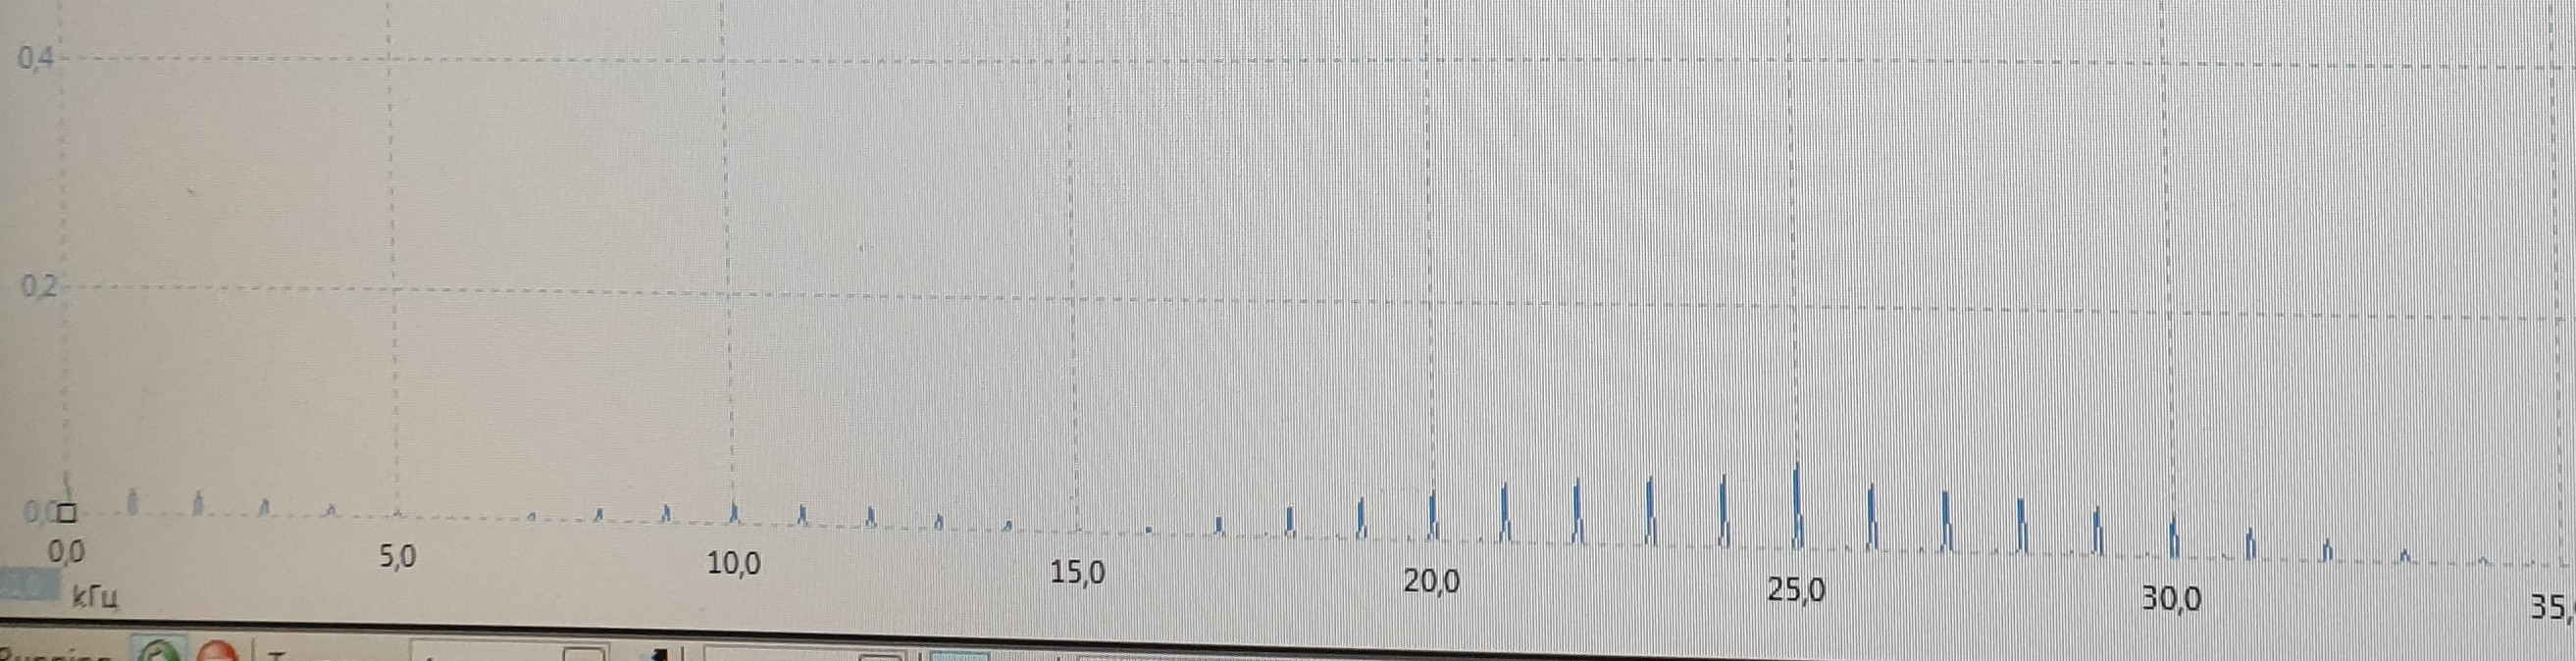
\includegraphics[width=0.6\textwidth]{cug_1.jpg}
    \caption{Спектр при \( \nu_{rep} = 1кГц, \nu_0 = 25 кГц, \tau = 100мкс\)}
    \label{spec_cug_1}
\end{figure}

\begin{figure}[H]
    \centering
    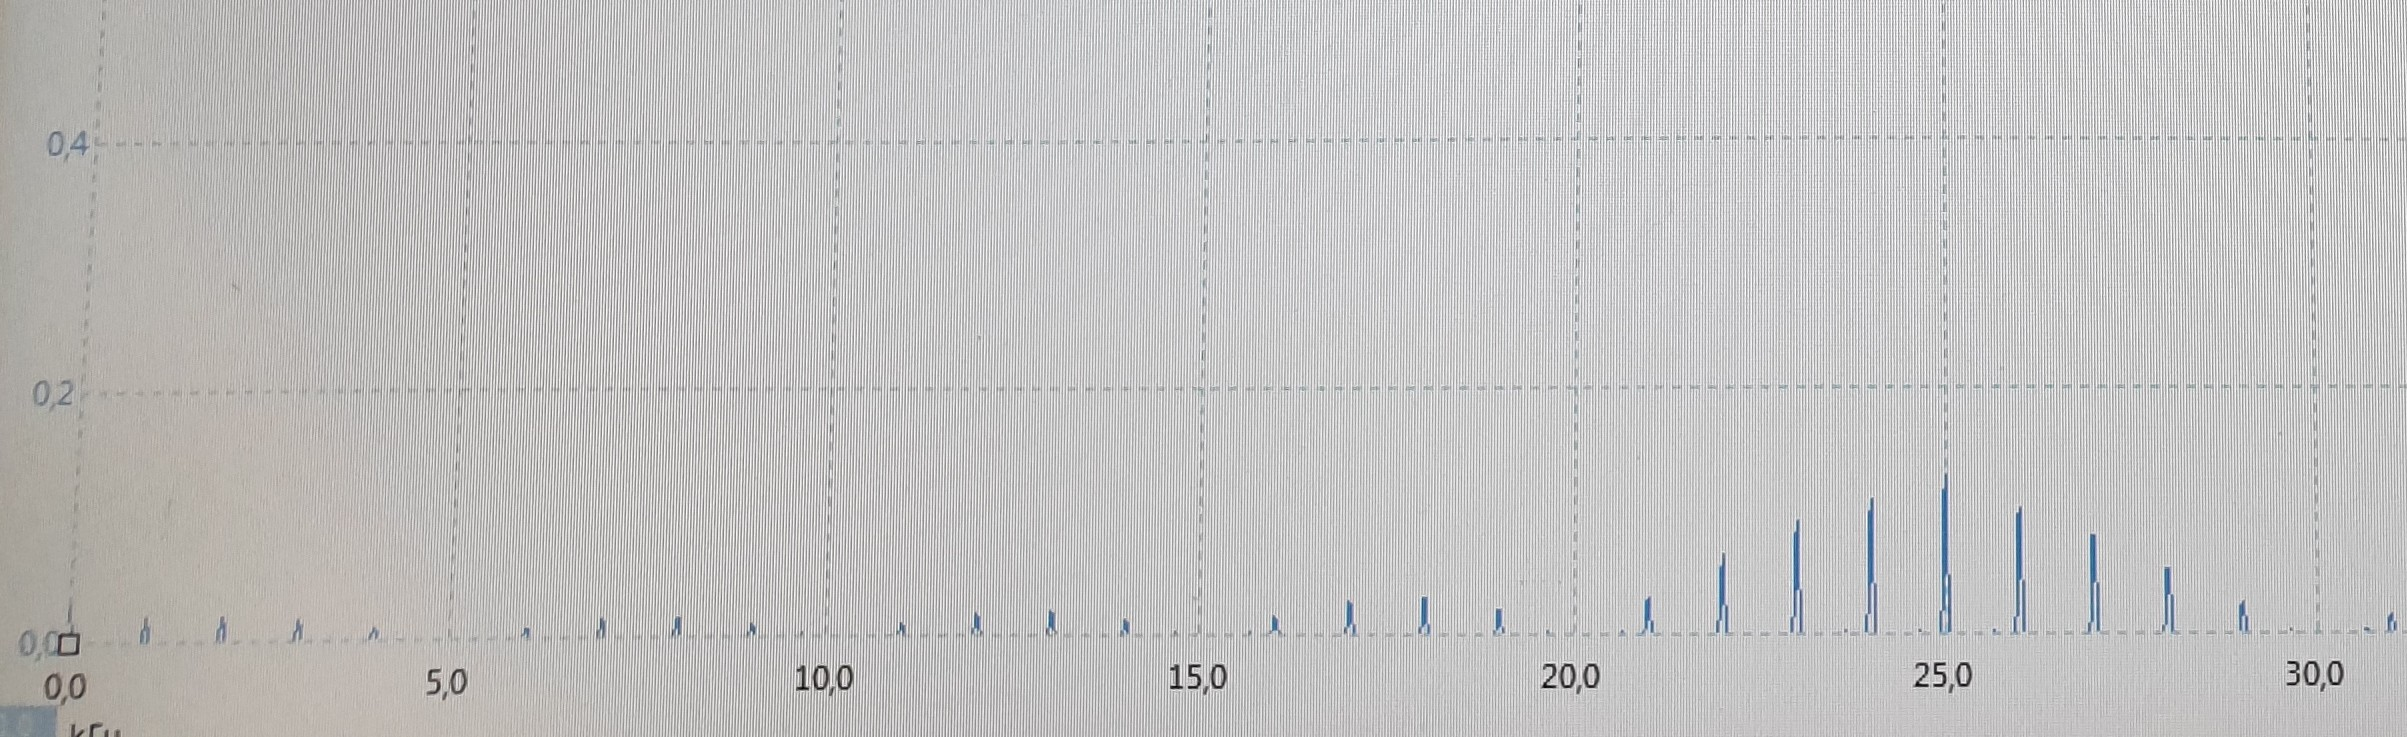
\includegraphics[width=0.6\textwidth]{cug_2.jpg}
    \caption{Спектр при \( \nu_{rep} = 1кГц, \nu_0 = 25 кГц, \tau = 200мкс\)} 
    \label{spec_cug_2}
\end{figure}

\begin{figure}[H]
    \centering
    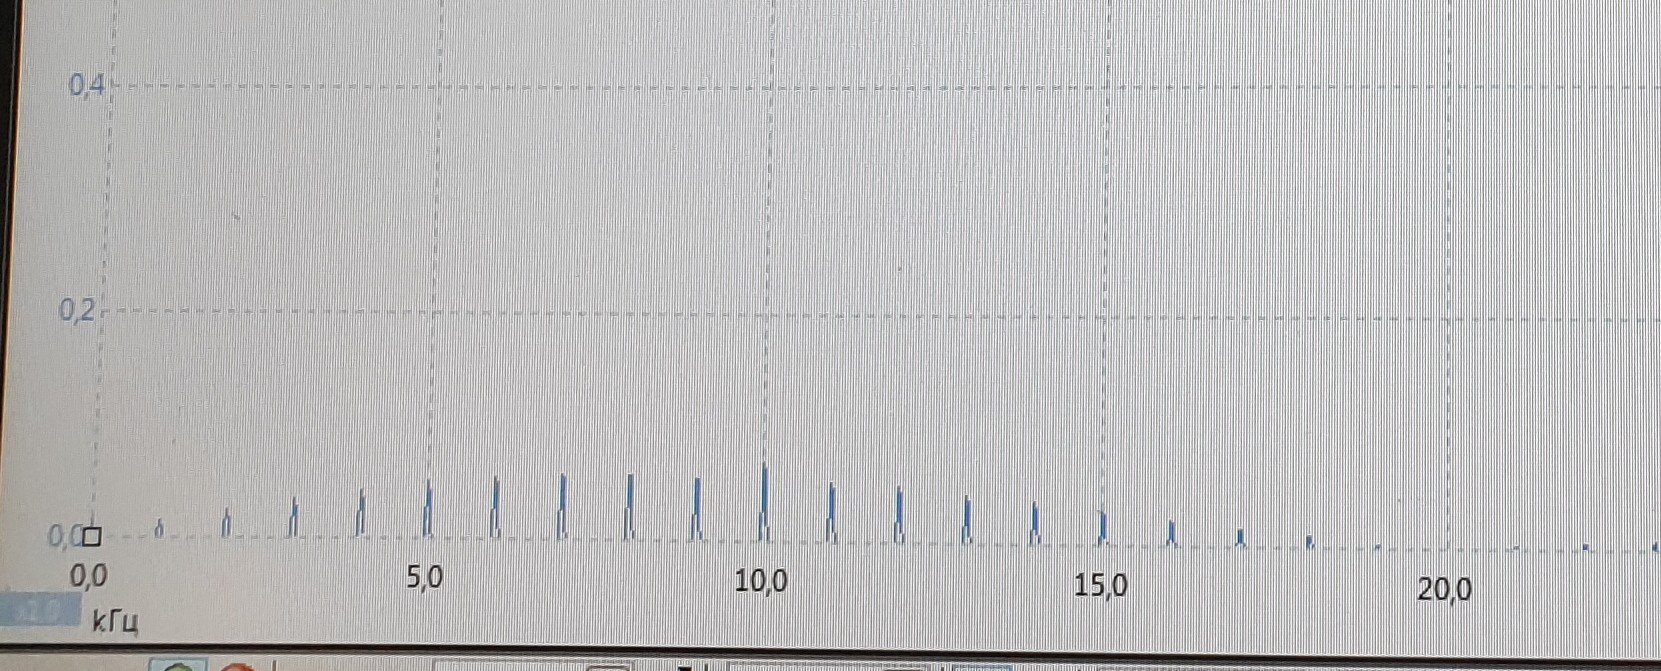
\includegraphics[width=0.6\textwidth]{cug_3.jpg}
    \caption{Спектр при \( \nu_{rep} = 1кГц, \nu_0 = 10 кГц, \tau = 100мкс\)} 
    \label{spec_cug_2}
\end{figure}

\begin{figure}[H]
    \centering
    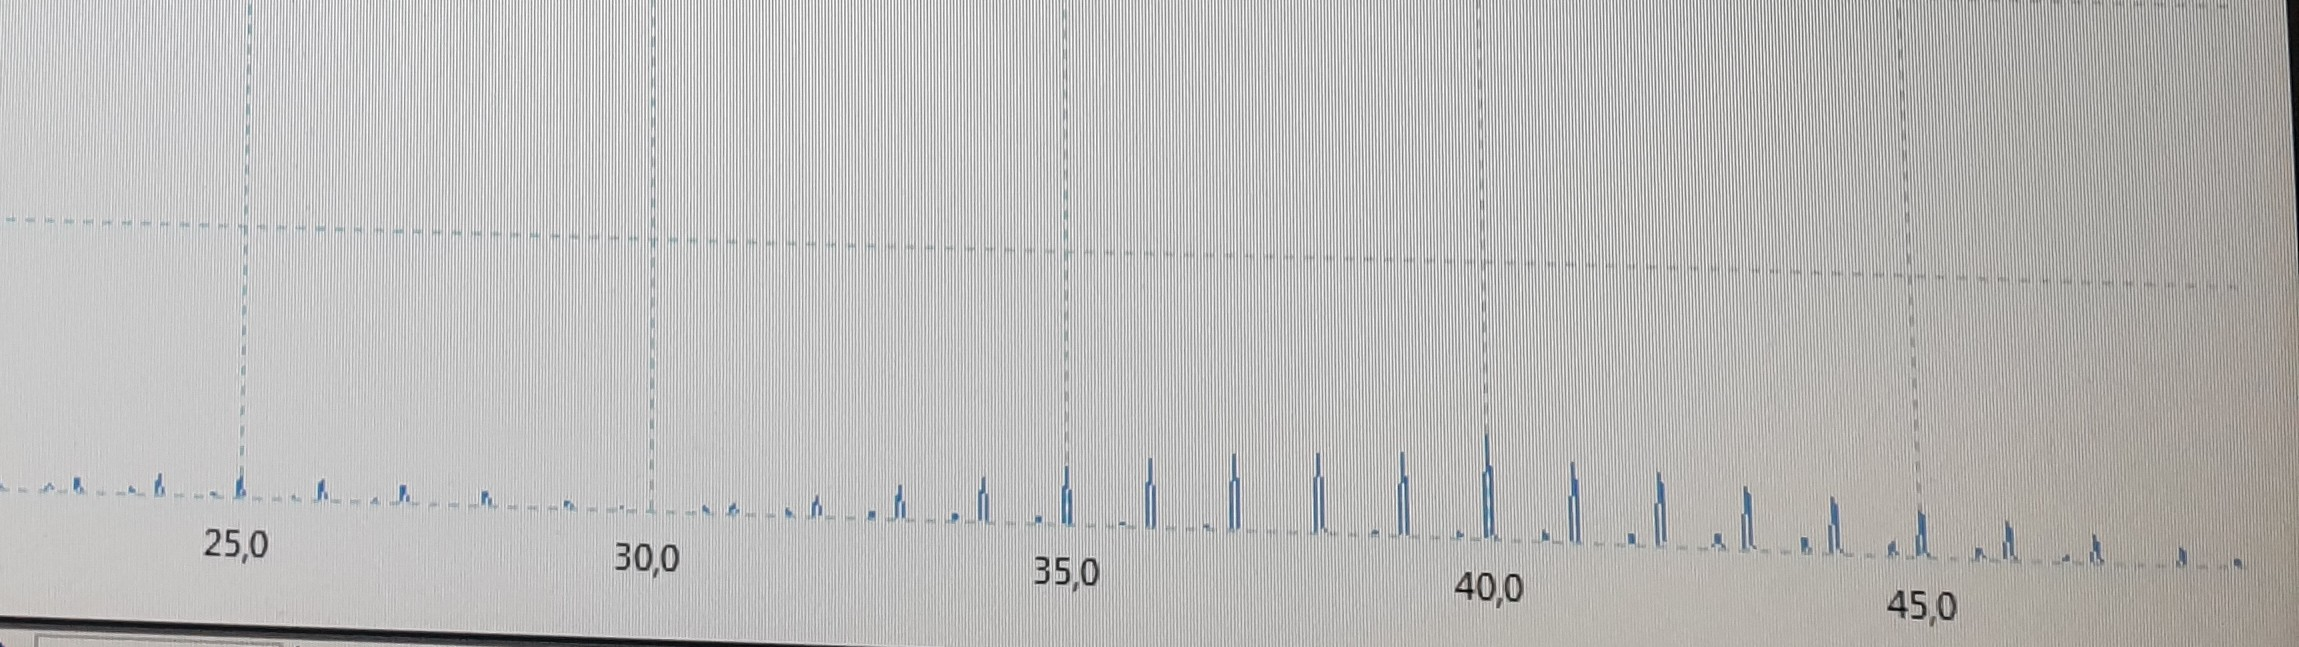
\includegraphics[width=0.6\textwidth]{cug_4.jpg}
    \caption{Спектр при \( \nu_{rep} = 1кГц, \nu_0 = 40 кГц, \tau = 100мкс\)} 
    \label{spec_cug_2}
\end{figure}

\begin{figure}[H]
    \centering
    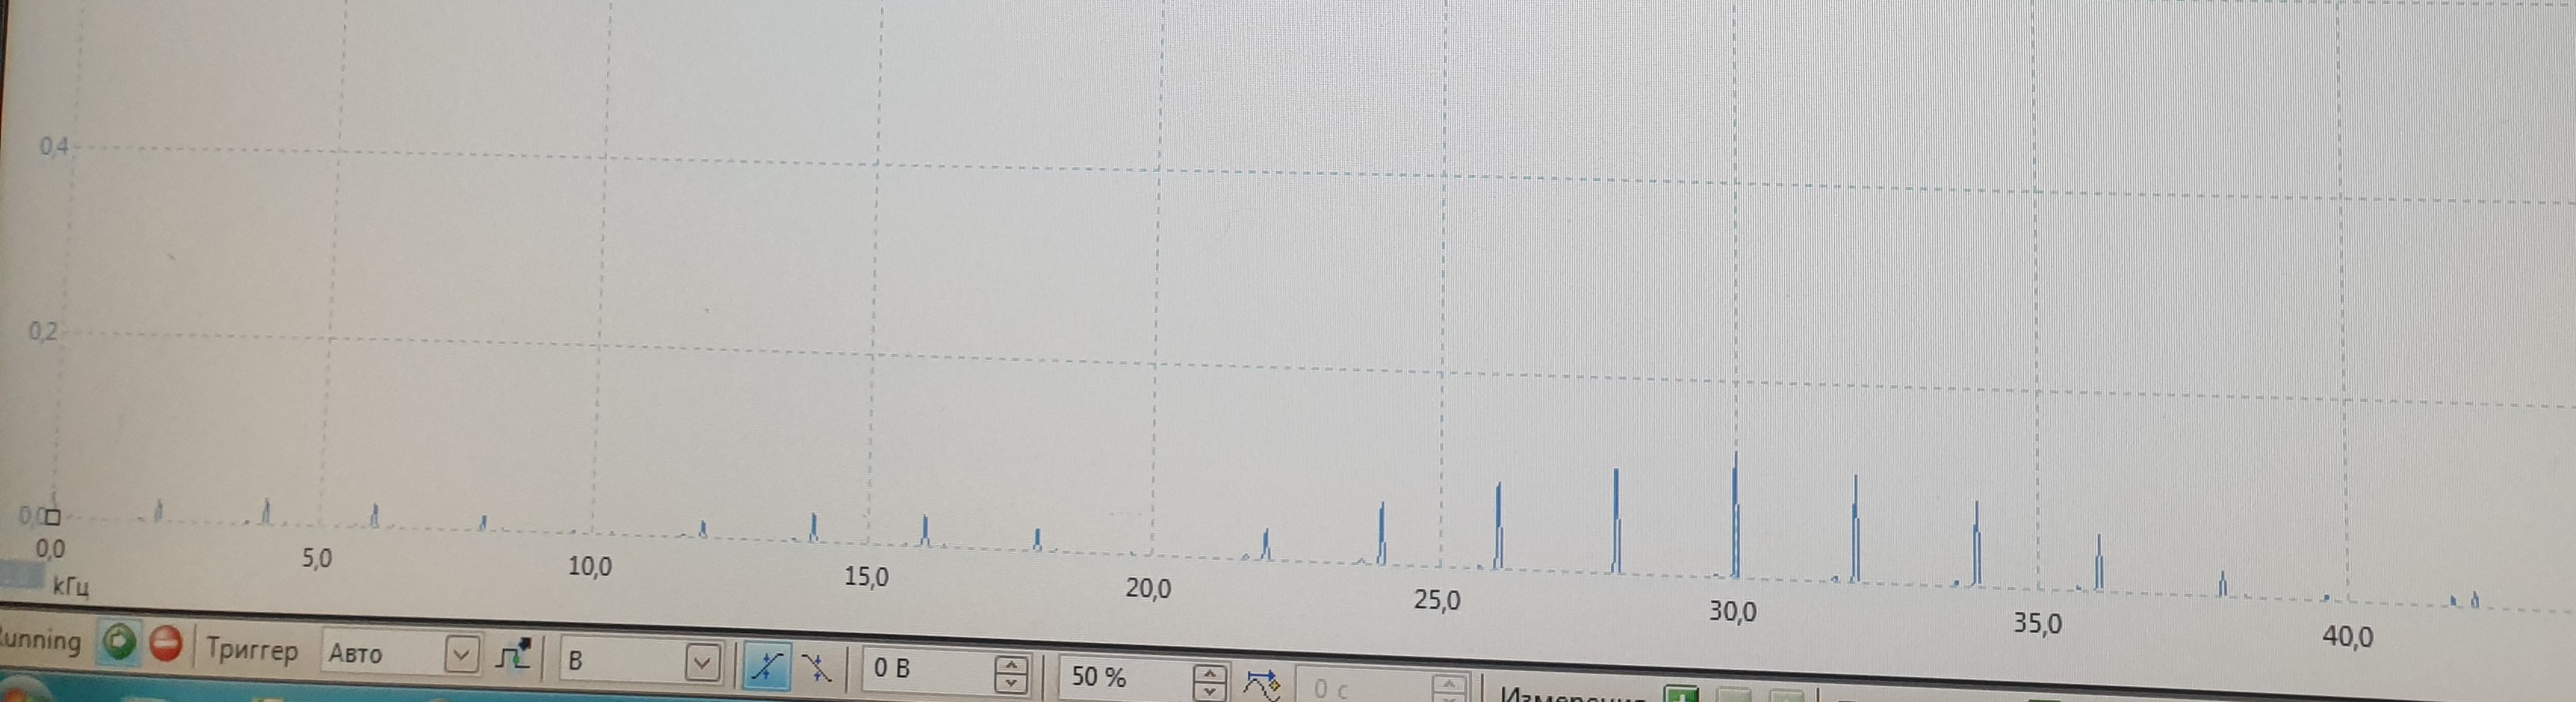
\includegraphics[width=0.6\textwidth]{cug_5.jpg}
    \caption{Спектр при \( \nu_{rep} = 2кГц, \nu_0 = 30 кГц, \tau = 100мкс\)}
    \label{spec_cug_1}
\end{figure}

Получим зависимость \( \delta\nu (\nu_{rep}) \) при \( \tau = 100\) мкс и \(\nu_0 = 25\) кГц:


\begin{table}[H]
    \centering
    \begin{tabular}{|c|c|}
        \hline
        \(\delta\nu\), кГц & \(\nu_{rep}\), кГц\\\hline
        0.5 & 0.5 \\\hline
        1   & 1   \\\hline
        2   & 2   \\\hline
        4   & 4   \\\hline
        5   & 5   \\\hline
    \end{tabular}
\end{table}

\begin{figure}[H]
    \centering
    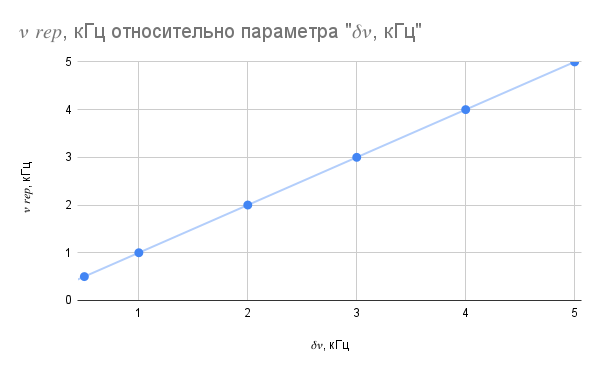
\includegraphics[width=0.8\textwidth]{graf2.png}
    \caption{График \( \delta\nu(\nu_{rep}) \) для прямоугольных импульсов с \( \nu_0 = 25\) кГц и \(\tau = 100\) мкс}
    \label{pic_dnu_tau}
\end{figure}

Получим завивисимость:

\[ \delta\nu = (1.0 \pm 0.1)\cdot\nu_{rep} + (0.0 \pm 0.1) кГц \]


Тоже выполняется соотношение неопределённости:
\[ \delta\nu\cdot T \simeq 1 \]


\subsection{C. Исследование спектра гармонических сигналов, модулированных по амплитуде}

Получим спектр исследуемого сигнала. Для этого установим частоту несущей \( \nu_0 = 25 \) кГц и частоту модуляции \( \nu_{mod} = 1 \) кГц.


\begin{figure}[H]
    \centering
    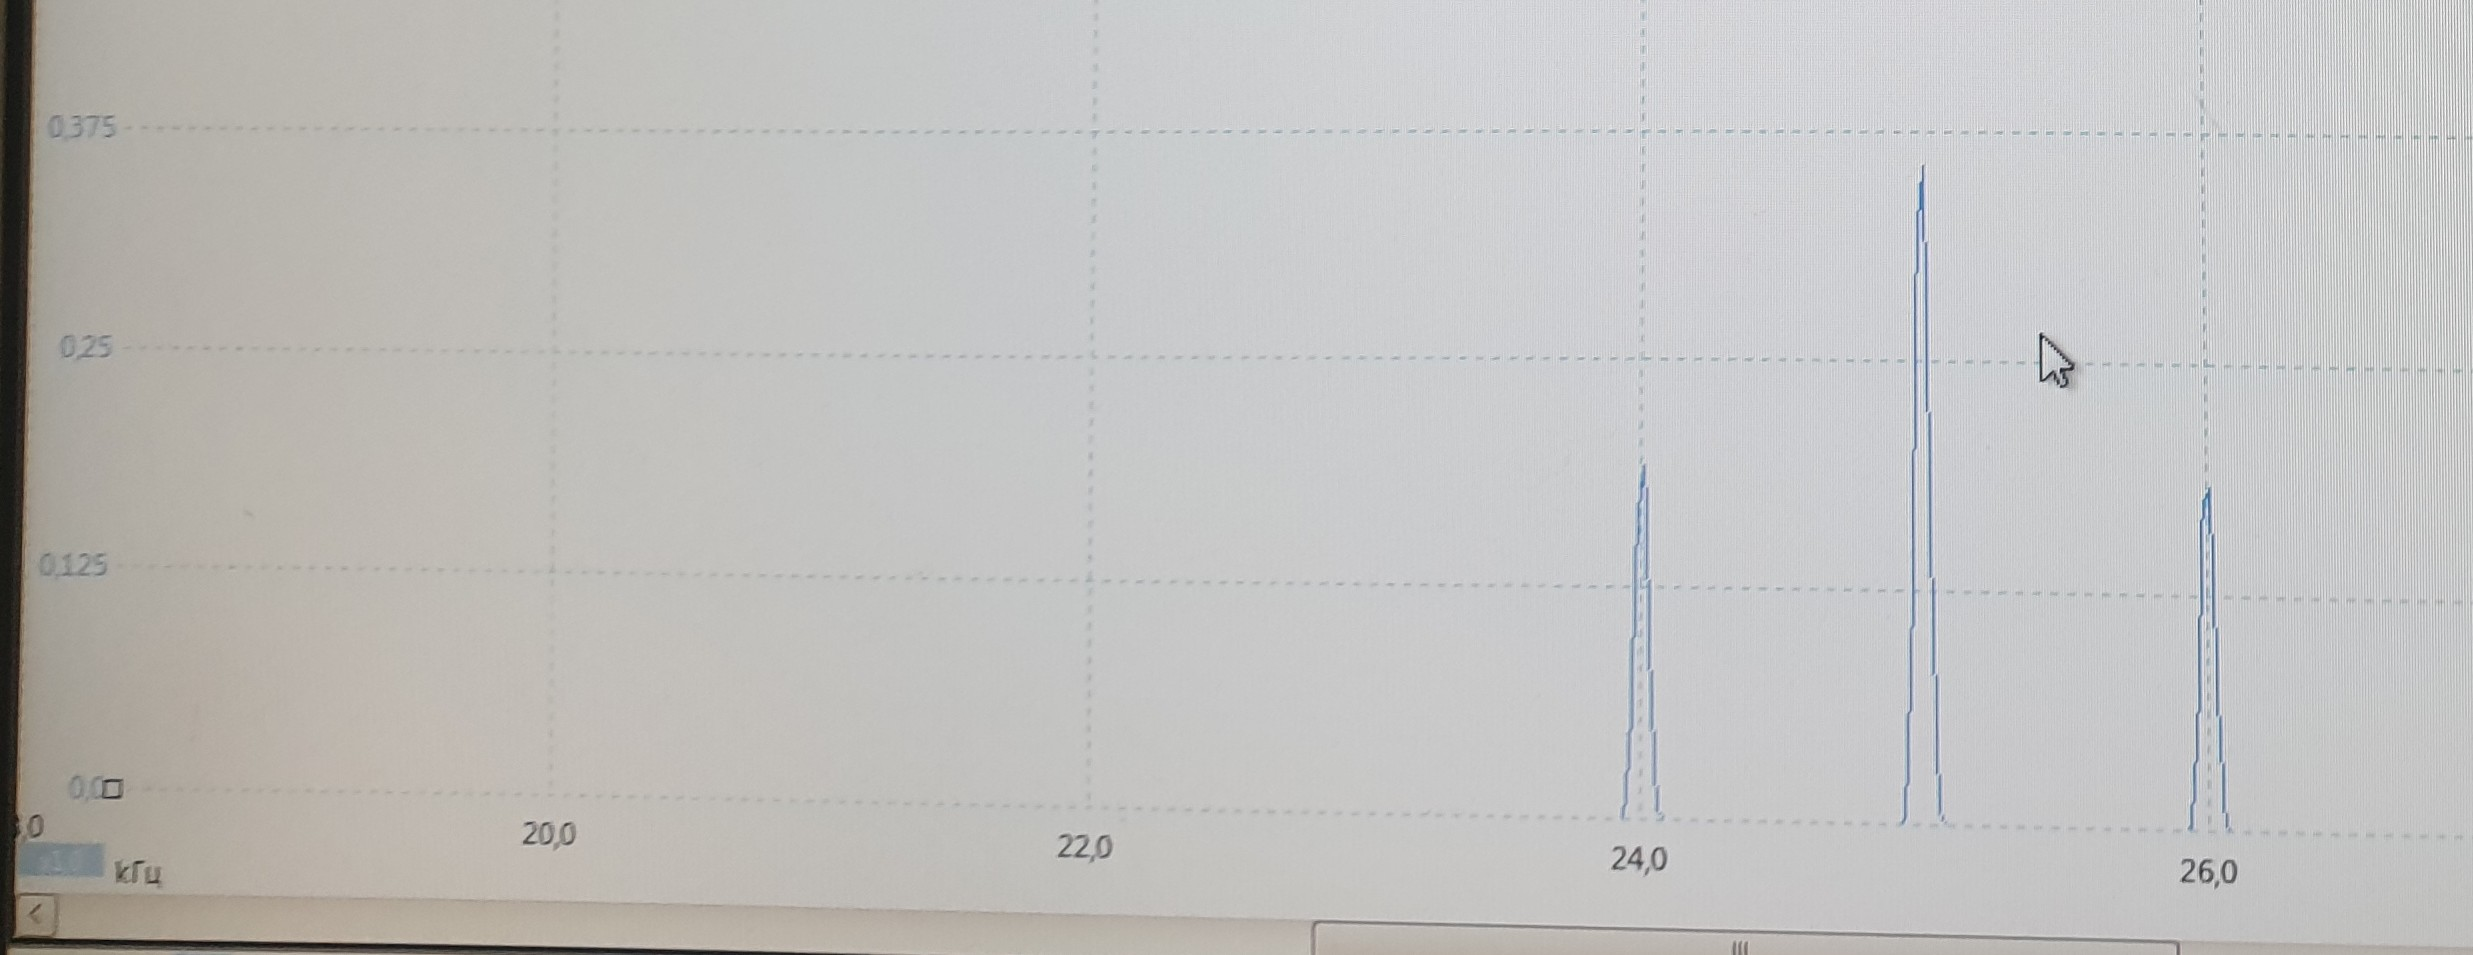
\includegraphics[width=0.8\textwidth]{mod_1.jpg}
    \caption{Спектр модулированного сигнала при \( m = 1 \).}
    \label{spec_mod}
\end{figure}

Изучим зависимость отношения амплитуд \( k = A_s/A_m \) боковой и основной частоты от 
параметра \(m = \left(A_{max} - A_{min}\right) / \left(A_{max} + A_{min}\right)\).


\begin{table}[H]
    \centering
    \begin{tabular}{|c|c|c|c|}
        \hline
        \(A_{m}\), mV &  \(A_{s}\), mV & \(m\) & \(k\) \\\hline
        322 & 16  & 0.1 & 0.050 \\\hline
        322 & 47  & 0.3 & 0.146 \\\hline
        322 & 75  & 0.5 & 0.233 \\\hline
        322 & 107 & 0.7 & 0.332 \\\hline
        322 & 139 & 0.9 & 0.431 \\\hline
        322 & 153 & 1.0 & 0.475 \\\hline
        \end{tabular}
\end{table}

\begin{figure}[H]
    \centering
    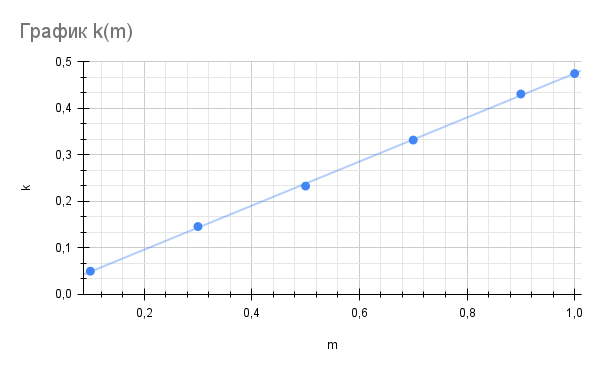
\includegraphics[width=0.8\textwidth]{graf3.png}
    \caption{График \( k(m) \) для модулированного сигнала с \(\nu_0 = 25\) кГц, \(\nu_{mod} = 1\) кГц}
    \label{pic_dnu_tau}
\end{figure}

Получим зависимость:

\[ k = (0.474 \pm 0.004)\cdot m + (0.001 \pm 0.001) \]


Установим, что 
\[ \frac{k}{m} = 0.474 \pm 0.04 \]

Это почти сходится с теорией (0,5).

\section{Выводы}

В лабараторной работе былт изучена зависимость спектра прямогольных сигналов, гармонических цугов и амплитудно модулированного гармонического сигнала. Также были прверены соотношения неорпеделенности, проверены справедливость разложения сигналов в ряд Фурье. Все сошлось с теорией.

\end{document}